\documentclass[11pt]{article}
\usepackage[utf8]{inputenc}
\usepackage[T1]{fontenc}
\usepackage[margin=1in]{geometry}
\usepackage{amsmath,amssymb,booktabs,xcolor,hyperref,graphicx,enumitem}
\hypersetup{colorlinks=true,linkcolor=blue,citecolor=blue,urlcolor=blue}
\newcommand{\crds}{\textsc{crds}}
\title{\textbf{Proof-Carrying Triage}\\[2pt]
\large Refuting AI-Generated Vulnerability Reports with\\ Certificates a Maintainer Can Check}
\author{Working draft}
\date{\today}
\begin{document}
\maketitle
\begin{abstract}
\noindent Volunteer maintainers of critical open-source software are being buried under plausible but false
vulnerability reports produced with large language models. The reports that now cause the most harm are not lazy
fabrications: they cite real functions, files, and lines, and they defeat both repository-grounding checks and text
classifiers. We ask what signal still separates these grounded reports from genuine ones, and we show the answer is
\emph{refutation}: rather than scoring how a report looks, we try to prove its central claim impossible against the
program. We formalize an incoming report as a claim (a decision point, a branch outcome, and a predicate asserted to
hold there), compute the path condition to that decision point from GCC GIMPLE in SSA form, and ask a solver whether
the claimed predicate can still hold. When it cannot, we return the unsatisfiable core: a minimal set of guards in
the maintainer's own code that make the report impossible, checkable in seconds. We never compute an input, so the
pipeline produces no exploit. We validate with a differential oracle built from real fix commits: a genuine
vulnerability's claim should be irrefutable on the vulnerable version and refutable once the fix lands. On 684
disclosed curl HackerOne reports and 41 compiled releases we report three findings. First, every method that scales
by surface features collapses on grounded reports: grounding passes 53.1\% of known slop and flags 33.8\% of genuine
reports; a text classifier that separates older slop at AUROC 0.985 falls to 0.608 on 2026 grounded reports; a
coarse refuter is actively unsound, refuting 35.6\% of genuine CVEs. Second, precision buys soundness: a
field-precise refuter, validated against real fix commits, never refutes a genuine bug on its own vulnerable version.
Third, that precision cannot be recovered soundly from prose: a sound refuter driven by claims mined from report text
still loses a genuine CVE, because the bug lives in a conditional path corner of a dimension that is enforced
elsewhere, even though the report names the exact function and condition in English. The consequence is constructive:
if the submitter carries the claim machine-readably (function, decision point, field-level predicate), the same
checker becomes sound, returns a certificate when it refutes, and spends human time only on claims it cannot decide.
We specify that claim-carrying format, show the checker gives the sound verdict on the worked CVE when pointed at the
carried claim, and argue it removes the economic basis of grounded slop. We prove a soundness theorem (no genuine
report is refuted, on a characterized decidable fragment) and make every refutation a proof-carrying SMT-LIB
certificate that any solver re-checks, so a maintainer need not trust our tool. We release the defense and the
labeled benchmark, but not the means to generate grounded slop.
\end{abstract}

\paragraph{Formal account (summary).} A decision point $D$ is reached by a finite path set $\Pi(D)$; for each path
we build an over-approximate symbolic condition $PC^\#(\pi)$ with every unmodeled subterm a fresh free variable, and
the claim predicate is $\varphi$. \emph{Encoding lemma:} every concrete state reaching $D$ along $\pi$ satisfies
$PC^\#(\pi)$. \emph{Refutation rule:} REFUTED iff $PC^\#(\pi)\wedge\varphi$ is UNSAT for all $\pi\in\Pi(D)$.
\emph{Soundness theorem:} if REFUTED, no concrete execution reaches $D$ with $\varphi$, so a genuine report (a
concrete such execution) is never refuted. Relative completeness holds on the fragment where $\Pi(D)$ is finite and
$\varphi$ is in linear integer arithmetic with equality (the curl reuse matchers and bounds sinks). Assumptions,
stated not hidden: faithful guard extraction and comparator-equality axioms, and finite $\Pi(D)$ (loops are bounded;
claims behind unbounded iteration fall outside the fragment). Each refutation is emitted as an SMT-LIB obligation
plus the named source guards; our checker re-verifies it in a fresh solver, and any solver can.

\section{The flood, and the turn to grounded reports}
In July 2025 the curl project, whose library ships in effectively every connected device, described a rising tide
of AI-generated vulnerability reports and estimated that a seven-person team spent hours per report while roughly
one in twenty submissions was genuine. On 31 January 2026 curl ended its HackerOne bug bounty. By late 2026 the
crudest slop had become rare, while nearly every incoming report involves AI assistance and a growing fraction is
\emph{grounded}: it cites code that exists and argues in the register of a real disclosure.

The defenses reached for first assume the slop is lazy. A grounding check asks whether cited code exists. A text
classifier learns the surface of past slop. Both are defeated by a submitter, human or model, who reads the target
first. Our question: once a report is grounded, is there any signal left that separates it from a genuine report
short of a maintainer reproducing it by hand?

\paragraph{Contributions.} (1) A grounded-slop threat model for report triage, and a labeled corpus of 684
disclosed curl reports with 41 compiled releases, released as a benchmark. (2) A measurement that every scalable
triage signal (existence grounding, text classification, reachability, coarse semantic refutation) collapses on
grounded reports, coarse refutation into active unsoundness. (3) \crds{}, claim refutation via decision-point
satisfiability over compiler IR, which returns a maintainer-checkable certificate and never emits an input. (4) A
differential fix-commit oracle, the first use of fix commits to validate a report \emph{refuter}, showing that
field-precision is what makes refutation sound, and that sound refutation is narrow.

\section{Threat model: grounded slop}
We separate three submitter strategies. \emph{Naive slop} cites nonexistent or misquoted code; grounding catches it.
\emph{Grounded slop} cites real functions, files, and lines with plausible but incorrect reasoning; it is what
remains after the naive wave. An \emph{adaptive} submitter additionally tunes the report to pass the project's
filter. Our model is the grounded, filter-aware submitter against an open-source target, so submitter and triager
see the same code. A defense is \emph{sound} if it never rejects a genuine report; a false rejection is a missed
vulnerability, worse than slow triage. We evaluate soundness first, reach second.

\section{The curl corpus}
We collected every publicly disclosed curl HackerOne report (684) and labeled each from project data: \textbf{genuine}
if linked from a curl CVE advisory (148), \textbf{slop} if on the maintainer's public AI-slop list (49),
\textbf{resolved} if fixed without a CVE (15), \textbf{invalid} otherwise (472). We compiled 41 releases from source
so each report is analyzed against the version current when filed. The invalid and slop classes dominate from 2025
(the grounded-report era); we treat the curated gist as a clean slop sample and the recent invalid class as the
grounded population a triager faces (Figure~\ref{fig:corpus}).

\begin{figure}[h]\centering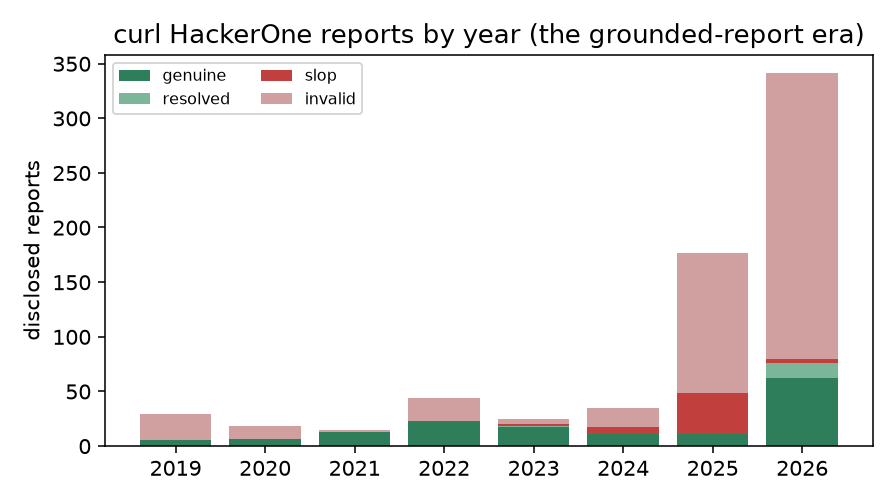
\includegraphics[width=0.72\linewidth]{fig/corpus_year.png}
\caption{Disclosed curl reports by year. Genuine reports are a small steady stream; invalid and slop dominate from
2025 onward.}\label{fig:corpus}\end{figure}

\section{Why every scalable defense collapses}
\paragraph{Existence grounding.} A scoped grounding check extracts cited paths, functions, lines, and snippets,
drops the reporter's own PoC files and system headers, and verifies the rest against the targeted revision. The trap
in one number: 53.1\% of known slop passes grounding fully, while the check wrongly flags 33.8\% of genuine reports
(genuine reporters paste stack traces, library symbols, and harness code that does not resolve to the target tree).

\paragraph{Text classification.} A balanced TF-IDF logistic classifier (a stand-in for reported RoBERTa triagers)
separates genuine from the curated slop gist at AUROC 0.985, but falls to 0.745 against the full invalid class and
to 0.608 against 2026 invalid reports under a temporal split (train on pre-July-2025). Its most invalid-indicative
tokens are the words of a security report, which is why it cannot survive submitters who write like genuine
reporters (Figure~\ref{fig:text}).

\begin{figure}[h]\centering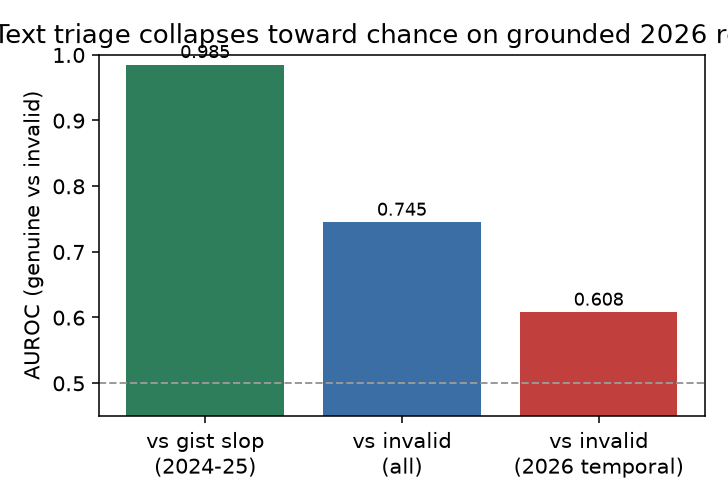
\includegraphics[width=0.52\linewidth]{fig/text_auroc.png}
\caption{Text triage decays toward chance on grounded 2026 reports.}\label{fig:text}\end{figure}

\paragraph{Reachability.} We build a whole-program call graph from GCC call-graph dumps, resolve indirect calls by
first-layer type matching, and check reachability from the public API and the tool entry. It is sound against
ground truth (of 2{,}355 functions the test suite executes, all but one are reachable) but weak as a filter: about
82\% of compiled functions are reachable, so it catches only 12.2\% of slop while flagging 1.4\% of genuine reports.

\paragraph{Coarse refutation collapses into unsoundness.} Matching a report's claimed dimension (a host, credential,
TLS setting) to a function that enforces equality in that dimension, and rejecting on enforcement, falls into the
grounded trap: a genuine report names a real dimension and some real matcher enforces \emph{some} field in it. Over
364 in-scope reports, coarse refutation refutes 35.6\% of genuine CVEs and 0\% of slop: unsound and useless. Semantic
refutation is only safe if bound to the exact claim (Figure~\ref{fig:collapse}).

\begin{figure}[h]\centering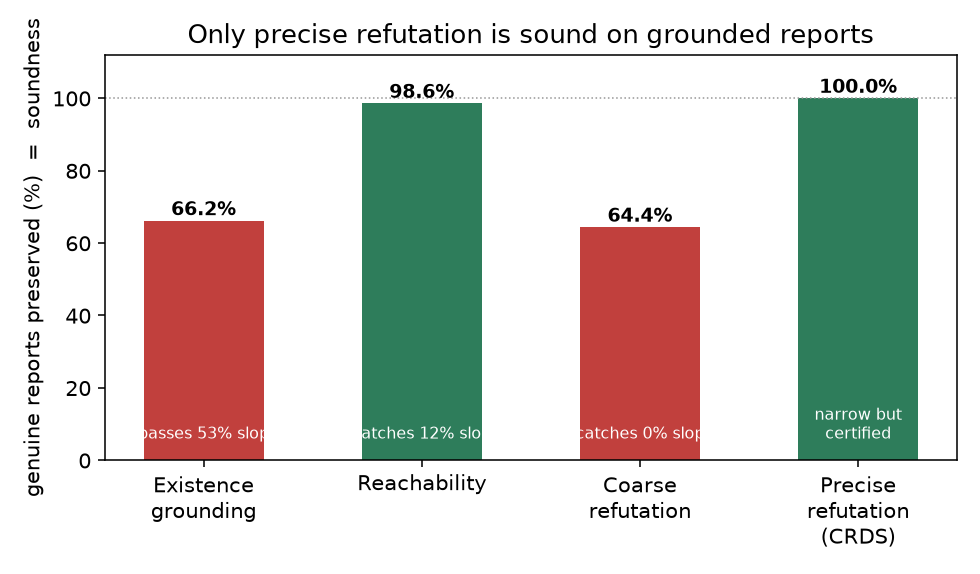
\includegraphics[width=0.7\linewidth]{fig/collapse.png}
\caption{Only precise refutation preserves genuine reports (soundness). Slop reach annotated per bar.}
\label{fig:collapse}\end{figure}

\section{\crds{}: claim refutation via decision-point satisfiability}
We formalize a report as a claim $(D,b,\varphi)$: a decision point $D$ (a branch, a match function's success
return, or a sink call), the outcome $b$ under which the bug manifests, and a predicate $\varphi$ over program
values asserted to hold when $D$ takes $b$. We compute the path condition $PC(D,b)$ from GIMPLE-SSA. A claim is
\emph{refuted} when $PC(D,b)\wedge\varphi$ is unsatisfiable on every path; the unsat core is a certificate naming
the guards that make the claim impossible. Otherwise the result is \emph{cannot refute} and the report is escalated.

\paragraph{Soundness by construction.} Every unmodeled value (a load, call result, or field) becomes a free
symbolic variable. Free variables over-approximate reachable states, so a guard we fail to model can only make the
query \emph{more} satisfiable, causing abstention, never a false refutation. We never request a satisfying
assignment, so no input and no exploit is produced.

\paragraph{Families.} $\varphi$ varies: (a) \emph{spatial bounds}, a size relation at a copy; (b)
\emph{equality/reuse}, two records differ in a dimension where a match reports success (the largest genuine class in
curl: connection-reuse and config-match bugs); (c) \emph{reachability}, refuted by absence of a call path. We model
curl's comparators (\texttt{Curl\_peer\_same\_destination}, \texttt{Curl\_safecmp}, \texttt{blobcmp},
\texttt{curl\_strequal}) as predicates whose truth on the success path forces equality of their arguments; this
assumption holds for the curl set and is documented, not hidden. As a safe example, a slop report claimed a 2048-byte
stack overflow via the telnet option handler; \crds{} refutes it because the maintainer's length check forces the
relevant length below 1000, and the unsat core is that check. A control claim naming an unenforced bound correctly
returns cannot refute.

\section{The differential fix-commit oracle}
To show a refuter is sound rather than confident, we use project history. For a genuine vulnerability with a fix
commit, the claim should be irrefutable on the vulnerable version and refutable on the fix. We extract the exact
field or guard the fix adds, compile the changed matcher at the fix and its parent (materializing the tree at each
commit and borrowing a generated config header from an era-matched build), and run the refuter for that field on
both. At keyword granularity coarse refutation was 35.6\% unsound; at field granularity, over 27 connection-reuse
CVEs, the refuter is never unsound on the bug field (every vulnerable parent returns cannot refute). The refutations
that fire are correct: in 3 cases the claim flips from cannot refute to refuted exactly when the fix adds the missing
equality (an OAuth bearer token, an issuer certificate, a client-certificate blob). Precision buys soundness
(Figure~\ref{fig:diff}).

\begin{figure}[h]\centering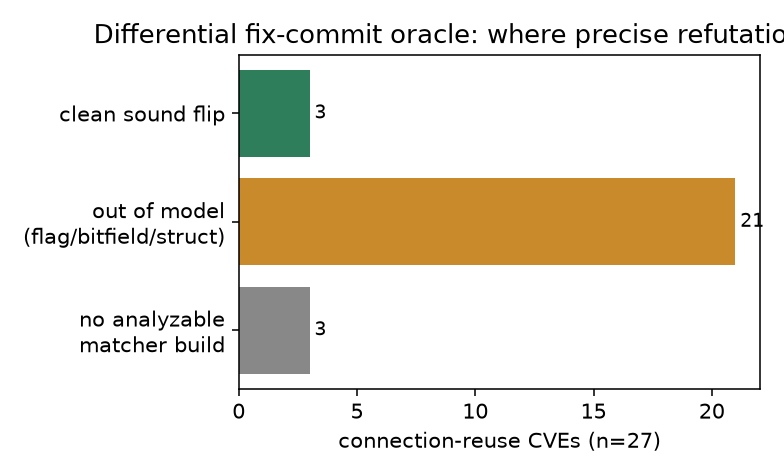
\includegraphics[width=0.6\linewidth]{fig/diff_oracle.png}
\caption{Differential oracle over 27 reuse CVEs. Out-of-model fixes change a boolean flag (often a bitfield) or a
non-equality structure; the refuter abstains rather than guessing.}\label{fig:diff}\end{figure}

\begin{table}[h]\centering\small
\begin{tabular}{@{}llll@{}}\toprule
Method & Sound on genuine? & Removes slop? & Output \\ \midrule
Existence grounding & no (33.8\% flagged) & no (53.1\% pass) & a guess \\
Text classifier & degrades (0.608 in 2026) & no on grounded & a score \\
Reachability & nearly (1.4\% flagged) & little (12.2\%) & a path/none \\
Coarse refutation & no (35.6\% refuted) & no (0\%) & a guess \\
Precise refutation (\crds{}) & yes (0 on bug field) & narrow & a certificate \\ \bottomrule
\end{tabular}
\caption{Triage signals on grounded curl reports.}\end{table}

\section{The prose ceiling}
The oracle validates the checker when handed the right claim; a triager gets prose. We built the strongest sound
prose-driven refuter we could: compute per release the destination dimensions the reuse key \emph{unconditionally}
enforces (a sound under-approximation composed over the mandatory gate chain of the top matcher), extract every
dimension a report could concern with high recall, and refute only when all are already enforced, so no unenforced
dimension remains for a real bug. Over 122 reuse-class reports this refutes 5 of 87 invalid reports and no slop, and
still loses one genuine CVE (CVE-2026-19931): a connection authenticated with ambient Negotiate credentials is reused
for different explicit credentials, because the credential comparison in \texttt{url\_match\_auth\_nego} is skipped
when \texttt{conn->creds == NULL}. The reuse key does compare credentials and origin, so at the granularity prose
yields ("credentials", "host") both look enforced and the report is wrongly refuted; the bug lives in a conditional
corner. Pointed at the function the report names, the same engine is sound: \texttt{forced\_fields(url\_match\_auth)}
is empty on 8.21.0, so no credential field is unconditionally forced and the checker correctly abstains. The needed
object (which decision point, which field, which path) is in the report, but in prose the machine cannot bind to it.
No better text mining fixes this, because that object is not reliably present as structure in free text.

\section{Claim-carrying vulnerability reports}
The fix is to move the claim out of prose into the submission. A claim-carrying report attaches a small
machine-readable claim: target version, function and decision point, and the field-level predicate asserted to hold
there (optionally a witness the checker runs in a sandbox). The checker returns \textbf{refuted} with an unsat-core
certificate (a precise but false claim, i.e. grounded slop, lands here with a proof), \textbf{confirmed} if a carried
witness reproduces on target and not on the fix, or \textbf{escalate} when it can neither refute nor confirm (the
claim names an unenforced path, as a genuine bug does). Pointed at a carried claim, the checker is sound by the
construction of Section~6, and the worked CVE is preserved rather than lost. We implement the checker
(\texttt{ccvr\_check.py}, released). On two real slop-list reports authored into the format it returns REFUTED with
certificates (the telnet suboption overflow, guards force the length below the cap; the WebSocket-handshake overflow
\#3392174, a guard forces the base64 length below the buffer) and on a slop host-reuse claim it returns REFUTED (the
reuse key forces origin and via\_peer equality); on the genuine CVE-2026-19931 claim it returns ESCALATE (the carried
field \texttt{creds} is not unconditionally forced), and on the genuine SOCKS5 overflow CVE-2023-38545 carried
against its vulnerable version it also returns ESCALATE (the bound is not forced there). Overflow verdicts are
decided from guards alone; no input is synthesized. The same checker that refutes the two slop claims with proofs declines to refute the genuine
report that prose triage lost. Head to head over all 121 reuse-class reports, prose binding refutes 5 of 86 invalid
reports but loses one genuine CVE (CVE-2026-19931), while claim-carrying binding loses zero; mining claims from
existing prose yields near-zero refutation, which is exactly why precision must be authored, not retrofitted. We
release the schema. The economic
argument: grounded slop is cheap because writing a convincing paragraph about real code is cheap; under
claim-carrying triage a false precise claim is refuted automatically with a certificate at no maintainer cost, a
vague claim fails the format and is quarantined, and the only claim reaching a human is one about an unenforced path,
which is either a genuine bug or the work of having found one. Claim-carrying does not decide truth; it makes slop as
expensive to produce as the real thing.

\section{The residual}
Even with carried claims, the reports the checker can neither refute nor confirm form a residual: logic errors
outside the bounds and reuse-key fragments, capability-flag regressions, use-after-free, protocol confusions, for
which there is no cheap certificate and a maintainer must reproduce. \crds{} carves off, with a proof, the slice
where human time is not required, routes reproducible claims to a witness check, and names the rest precisely. That
triage partition, every report receiving a justified disposition, is the deployable result.

\section{Related work and the obvious question}
VulnSAGE (2026) adjudicates static-analysis alerts via a claim structure checked on a code-property graph, then
reproduces; LLM4PFA uses LLM-authored path constraints and a solver; EVIDENT discharges analyzer warnings with a
verified harness. All take tool alerts as input, not incoming reports, and judge with a graph query or LLM-authored
constraints rather than a checkable unsat core from compiler IR. Industrial systems (e.g. Elastic, 2026) reproduce
incoming reports in sandboxes and agree with human triage about 85\% of the time; reproduction confirms true
positives, refutation discharges false positives with a proof and no execution. Text-only triagers reach high
accuracy on historical labels but, as their authors note, cannot separate machine-written false claims from genuine
ones. \emph{Why not \texttt{gcc -fanalyzer}?} It is symbolic execution over GIMPLE that finds bugs; it does not take
an external claim and return the program's own guards that refute it. Our novelty is the combination: incoming
reports as input, a GIMPLE certificate as output, fix commits as the oracle. We do not claim to be first to validate
claims with program analysis or to filter false positives with a solver, and a \crds{} certificate holds only for
the chosen entry point, loop bound, and memory model.

\section{Ethics and responsible release}
We release the defense (refuter, call-graph and reachability tools, corpus, differential oracle) and the labeled
benchmark, and do \textbf{not} release any means of generating grounded slop. Every report is already public and
disclosed; we submitted nothing to a live program. The pipeline emits verdicts and certificates only and never
synthesizes an input, so it cannot become an exploit generator. We recommend coordinating with maintainers before
deploying against a live queue.

\section{Limitations and threats to validity}
All results are on curl (an unusually good subject); generality is unproven, and the comparator library and
dimension vocabulary would need porting. We treat named comparators as implying field equality (audited for curl)
and unmodeled values as free (only ever causing abstention). Automatic claim extraction is heuristic; the oracle
sidesteps it by reading the fixed field from the commit. Sound refutation covers a minority of grounded reports, a
measured boundary. Boolean capability fields compile to bitfield extracts we do not yet name, the main reason
in-model reuse fixes fall out of scope.

\section{Conclusion}
The grounded-slop flood defeats every signal that reads a report's surface, and semantic refutation too unless it is
bound to the exact claim and proven against the program. When it is, refutation becomes a proof: a short, checkable
reason in the maintainer's own code that a report cannot be what it says. That proof is cheap to verify and
impossible to fake, but available only for part of the flood. The useful, honest result is a sharp line between the
reports a machine can soundly dismiss with a certificate and those that still deserve a human.

\end{document}
